\section{Results}
\label{sec:results}

\subsection{Nose wave drag}

Figure~\ref{fig:cdw}a gives the wave drag of the seven profiles at $L/D=4$ and
Figure~\ref{fig:cp} the wall pressure behind it. The wall pressure is shown as the pressure
coefficient $C_p = (p-p_\infty)/q_\infty$. By Equation~\eqref{eq:cdw}, $C_{D,\rm w}$ is the integral
of $C_p$ weighted by the forward-facing projected area of each surface element: regions of the nose
with $C_p > 0$ add drag, and regions with $C_p < 0$ reduce it.
\begin{itemize}[leftmargin=*,itemsep=2pt]
\item \textbf{Von K\'arm\'an and power $n=\tfrac12$ are the two low-drag profiles}, within a few
per cent of each other: Von K\'arm\'an is lower at $M \geq 1.3$, power $\tfrac12$ is lower at
$M \leq 1.2$. They get there differently. The tangent profiles (Von K\'arm\'an, ogive, parabolic)
expand continuously, and their wall pressure falls below ambient over the aft third. This
partly cancels the overpressure near the tip. The power-$\tfrac12$ nose concentrates its
overpressure in a short spike at its blunt tip and stays just above ambient behind it. On a
tangent profile the flow keeps expanding around the convex surface, and the aft part of the nose
still faces slightly forward, so the suction there acts as a small thrust.
\item \textbf{Ogive, parabolic and LV-Haack} carry 13--22\,\% more wave drag: their fuller
forebody turns the flow harder near the tip. The larger surface angle over the front third
compresses the flow more strongly, which shows as the higher $C_p$ of these shapes between
$x/L \approx 0.1$ and 0.4 in Figure~\ref{fig:cp}b.
\item \textbf{The cone is the worst} at every Mach number, and its drag rises steeply towards
Mach 1. Its surface pressure is the conical-flow value all the way to the shoulder. The surface
angle is constant, so nothing along the nose relieves the overpressure, and the whole turn back to
the axial direction happens in one expansion at the shoulder.
\item \textbf{Fineness.} $C_{D,\rm w}$ falls as $1/(L/D)^2$ for every profile, the slope of
slender-body theory (Figure~\ref{fig:cdw}b). For Von K\'arm\'an the Euler level is about
15\,\% below the linear-theory value $1/(L/D)^2$. Linear theory therefore reproduces the trend
(Equation~\eqref{eq:fineness}) but not the level, which is why it is used here only to select the
candidates and to interpolate between fineness ratios (Section~\ref{sec:check45}).
\end{itemize}

\begin{figure}[H]
\centering
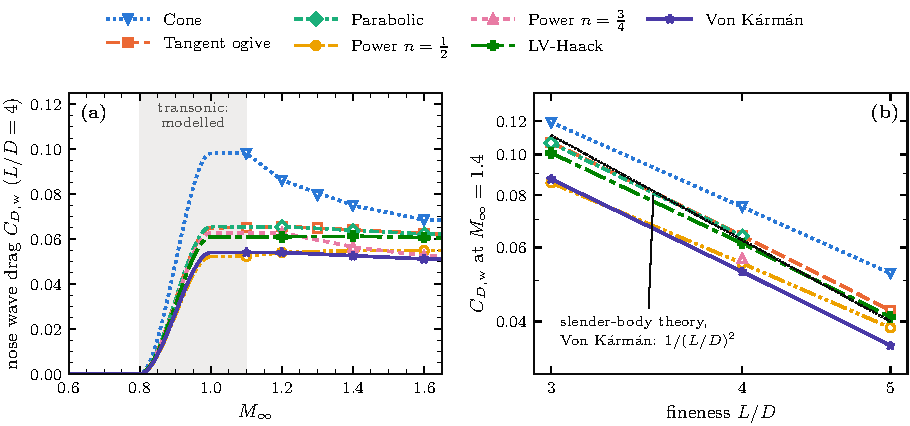
\includegraphics[width=\textwidth]{fig_cdw}
\caption{(a) Nose wave drag versus Mach number at $L/D=4$ (markers: Euler; lines: model used in
the trajectory; grey band: transonic model). (b) Wave drag versus fineness at $M=1.4$, with the
slender-body result for the Von K\'arm\'an nose.}
\label{fig:cdw}
\end{figure}

\begin{figure}[H]
\centering
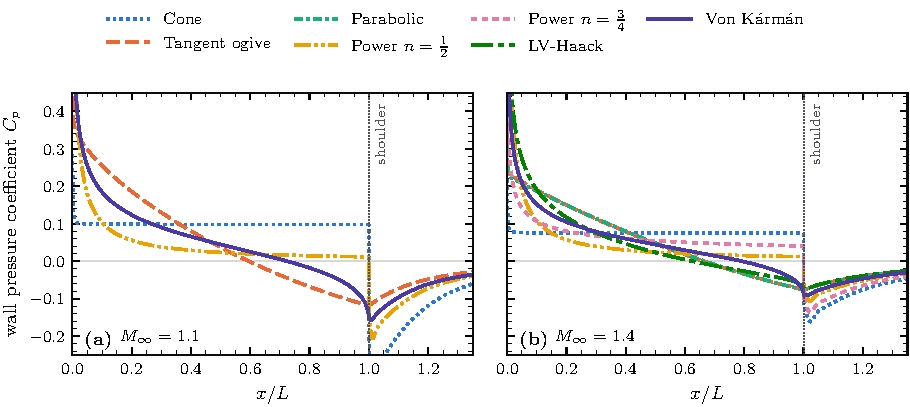
\includegraphics[width=\textwidth]{fig_cp}
\caption{Wall pressure coefficient along the nose ($L/D = 4$) at (a) $M=1.1$ (only the shapes
computed at that Mach number) and (b) $M=1.4$. The tangent profiles reach $C_p<0$ over the aft
third; the power-$\tfrac12$ nose keeps a small overpressure up to the shoulder after a spike at
its blunt tip; the cone keeps the conical value.}
\label{fig:cp}
\end{figure}

Figures~\ref{fig:cdw} and~\ref{fig:cp} show that, at a given length, the drag is decided by the
pressure distribution: shapes that compress the flow gently and then expand it along the rest of
the nose have the lowest drag. They also show that length is as powerful as shape. Going from
$L/D = 4$ to 4.5 lowers the Von K\'arm\'an wave drag at $M = 1.4$ by 19\,\% (0.0526 to 0.0425),
close to the factor $(4/4.5)^2 = 0.79$ of Equation~\eqref{eq:fineness}; at equal length, the
ogive carries 21\,\% more than the Von K\'arm\'an nose. The design question is therefore how to
combine the best profile with the longest nose the vehicle can accommodate.

\subsection{Flight performance}

Figure~\ref{fig:trajectory}a shows the nominal and envelope ascents. Weisshorn burns out at
\SI{9.1}{s} near \SI{2.2}{km} at $M_{\max}=1.47$ (nominal) or 1.56 (envelope). It spends \SI{16}{s} above $M = 0.8$ and
\SI{10}{s} above Mach 1. Figure~\ref{fig:trajectory}b shows where the drag impulse
$\int D\,\mathrm dt$ is spent: mostly between $M = 0.8$ and 1.5, which is exactly where the
nose wave drag acts. The apogee sensitivities around the baseline are
\textbf{\SI{-100}{m} per $\Delta C_D = 0.01$} and \textbf{\SI{-143}{m/kg}}.

The vehicle accelerates during the burn and then decelerates under drag and gravity. It crosses
the transonic band twice, once accelerating and once coasting (Figure~\ref{fig:trajectory}a).
The drag impulse, the integral of the drag force over time, is the momentum the vehicle loses to
drag. It is concentrated at high Mach number because the dynamic pressure is highest there (high
speed at low altitude), which is why a drag saving above $M = 0.8$ is worth so much apogee. The two
sensitivities convert any drag or mass difference into apogee. The $C_D$ sensitivity applies
to a change over the whole flight. A wave-drag difference only acts above $M = 0.8$ and is
therefore worth somewhat less: the ogive carries 0.009 more $C_{D,\rm w}$ than Von K\'arm\'an at
$M = 1.4$ and $L/D = 4.5$, and loses \SI{79}{m} rather than \SI{90}{m}.

\begin{figure}[H]
\centering
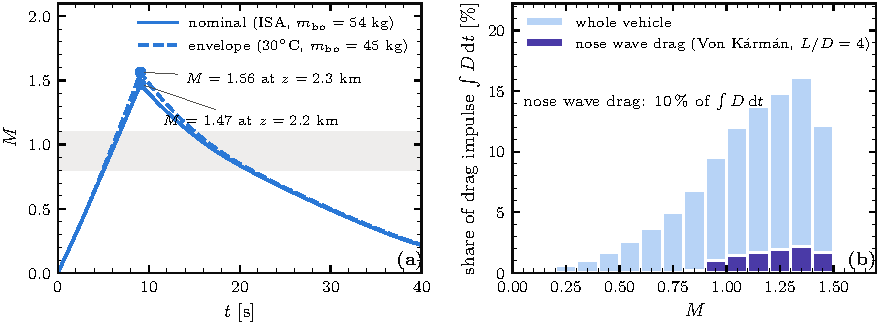
\includegraphics[width=\textwidth]{fig_trajectory}
\caption{(a) Mach number along the nominal and hot-day envelope ascents (grey band: transonic
range). (b) Share of the drag impulse per Mach bin for the baseline nose; the dark part is the
nose wave drag.}
\label{fig:trajectory}
\end{figure}

Figure~\ref{fig:breakdown} breaks the vehicle drag down by component for the recommended nose.
Skin friction dominates at all speeds (Weisshorn is a fineness-30 airframe). Base drag is the
second contributor, and the nose wave drag appears above $M = 0.8$, where it is 10--12\,\% of the
total. This is why the nose shape moves the apogee by tens of metres rather than kilometres, and
why the length (wetted area) and the shape effects are of the same order. A fineness-30 airframe
(\SI{5.4}{m} long for \SI{0.18}{m} in diameter) has a large wetted area for its frontal area, so
friction outweighs the pressure drag terms. The total drag coefficient peaks just above $M = 1$,
where the base, fin and nose pressure drags are all near their maximum.

\begin{figure}[H]
\centering
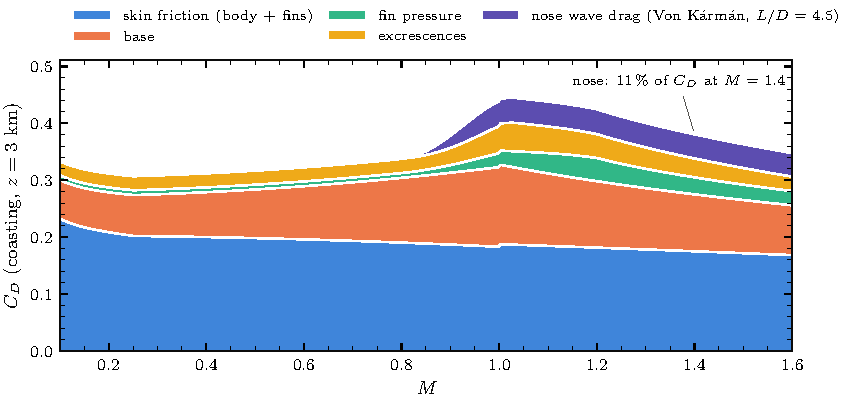
\includegraphics[width=\textwidth]{fig_breakdown}
\caption{Drag build-up of Weisshorn with the recommended nose (coasting, $z = \SI{3}{km}$, rest of
the vehicle scaled by the calibration factor $k$). The kink at $M\approx0.25$ is where the skin
friction becomes roughness-limited; the one at $M=1$ is the switch of the base-drag law.}
\label{fig:breakdown}
\end{figure}

\subsection{Trade study}
\label{sec:trade}

Figure~\ref{fig:trade} gives, for every profile and fineness, the apogee change relative to the
baseline, the length over which a 3U section fits, and the change in static margin.
Table~\ref{tab:trade} lists the candidates closest to the LVS length. Each point of
Figure~\ref{fig:trade}a is a full trajectory with the wave drag of that nose, its own length,
wetted area and shell mass. The curves rise with fineness because the wave drag falls as
$1/(L/D)^2$. They flatten because the friction and mass of the longer nose grow linearly with $L$.

\begin{figure}[H]
\centering
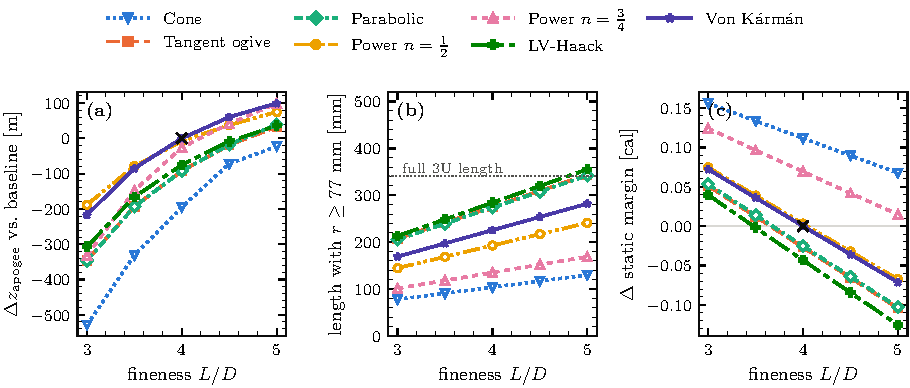
\includegraphics[width=\textwidth]{fig_trade}
\caption{(a) Apogee change relative to the baseline (Von K\'arm\'an, $L/D=4$, cross), including
the extra length, wetted area and mass of longer noses. (b) Length of the curved nose with
$r\geq\SI{77}{mm}$ (3U fit). (c) Change in subsonic static margin.}
\label{fig:trade}
\end{figure}

\begin{table}[H]
\centering
\caption{Candidates at $L/D=4$ (LVS length, \SI{720}{mm}) and $L/D=4.5$ (\SI{810}{mm}). $\Delta z$: apogee change vs.\ the baseline (Von K\'arm\'an, $L/D=4$); mass: shell + Al tip; 3U in nose: curved length with $r\geq\SI{77}{mm}$; bay: curved length plus the cylinder the 3U still needs.}
\label{tab:trade}
\small
\begin{adjustbox}{max width=\textwidth}
\begin{tabular}{@{}llcccccccc@{}}
\toprule
$L/D$ & Profile & \multicolumn{3}{c}{$C_{D,\rm w}$ at $M=$} & $\Delta z$ & mass & 3U in nose & bay & $\Delta$SM \\
 & & 1.1 & 1.2 & 1.4 & [m] & [g] & [mm] & [mm] & [cal] \\
\midrule
4 & Cone & 0.0982 & 0.0862 & 0.0750 & -195 & 261 & 104 & 966 & +0.11 \\
4 & Tangent ogive & 0.0651 & 0.0657 & 0.0640 & -93 & 328 & 275 & 795 & -0.03 \\
4 & Parabolic & 0.0656 & 0.0656 & 0.0639 & -92 & 328 & 274 & 797 & -0.03 \\
4 & Power $n=\tfrac12$ & 0.0523 & 0.0541 & 0.0550 & -8 & 328 & 193 & 878 & +0.00 \\
4 & Power $n=\tfrac34$ & 0.0628 & 0.0628 & 0.0564 & -26 & 289 & 135 & 935 & +0.07 \\
4 & LV-Haack & 0.0610 & 0.0610 & 0.0613 & -75 & 341 & 284 & 786 & -0.04 \\
4 & \textbf{Von K\'arm\'an} & 0.0541 & 0.0541 & 0.0526 & +0 & 321 & 226 & 845 & +0.00 \\
\midrule
4.5 & Cone & 0.0708 & 0.0708 & 0.0619 & -72 & 286 & 117 & 1043 & +0.09 \\
4.5 & Tangent ogive & 0.0530 & 0.0530 & 0.0516 & -19 & 361 & 309 & 870 & -0.07 \\
4.5 & Parabolic & 0.0529 & 0.0529 & 0.0515 & -18 & 361 & 308 & 870 & -0.06 \\
4.5 & Power $n=\tfrac12$ & 0.0450 & 0.0450 & 0.0457 & +38 & 361 & 217 & 943 & -0.03 \\
4.5 & Power $n=\tfrac34$ & 0.0513 & 0.0513 & 0.0463 & +42 & 318 & 152 & 1008 & +0.04 \\
4.5 & LV-Haack & 0.0496 & 0.0496 & 0.0497 & -9 & 376 & 320 & 870 & -0.08 \\
4.5 & \textbf{Von K\'arm\'an} & 0.0437 & 0.0437 & 0.0425 & +60 & 354 & 254 & 907 & -0.04 \\
\bottomrule
\end{tabular}
\end{adjustbox}
\end{table}


\begin{itemize}[leftmargin=*,itemsep=2pt]
\item \textbf{Von K\'arm\'an, power $\tfrac12$ and power $\tfrac34$ lead at every length} and swap
places within about \SI{30}{m}. Power $\tfrac12$ is ahead at $L/D\leq3.5$, Von K\'arm\'an at
$L/D = 4$--4.5, and the power-$\tfrac34$ estimate (scaled from $L/D=4$) at $L/D=5$. At $L/D=4$,
Von K\'arm\'an beats the tangent ogive (Bella Lui II / Nordend) by \TRADEOGIVE{} and the Firehorn
power-$\tfrac12$ by \TRADEPOWER{}.
\item \textbf{Length pays, with diminishing returns}: \TRADELEN{} per extra \SI{90}{mm}
($\Delta L/D = 0.5$) around $L/D = 4$--4.5.
\item \textbf{Fuller noses house more payload}: at $L/D=4$ the ogive and LV-Haack fit
\SIrange{275}{284}{mm} of the 3U inside the curved part, against \SI{226}{mm} for Von K\'arm\'an. Measured
as nose-bay length (curved part + the cylinder still needed for the 3U), the Von K\'arm\'an
nose still gives the highest apogee per millimetre of bay length. In Figure~\ref{fig:trade}b
only the fullest noses at $L/D = 5$ approach the full 3U length (dotted line).
\item \textbf{Stability is not a discriminator}: all candidates change the static margin by
less than 0.1 cal. A longer nose lowers the margin slightly (Figure~\ref{fig:trade}c): its CP,
a distance $V/A_b$ ahead of the shoulder, moves forward with $L$ faster than its extra mass moves
the CG. The largest change over the whole design space, 0.16 cal, is small against the 2--4 cal
target.
\end{itemize}

The trade study thus separates two groups: the low-drag group (Von K\'arm\'an and the power noses)
and the high-volume group (ogive, parabola, LV-Haack). Section~\ref{sec:selection} weighs drag
against payload room and manufacturing.

\subsection{Check at the design fineness}
\label{sec:check45}

The trade study interpolates the Euler results between $L/D = 3$, 4 and 5 (on $C_{D,\rm w}(L/D)^2$,
which is nearly constant for slender noses). To check this, every shape was also computed directly
at $L/D = 4.5$ (Table~\ref{tab:check45}). Where three fineness ratios were available the
interpolation is within 0.3\,\%. The parabolic and power-$\tfrac34$ noses, first computed at
$L/D = 4$ only, were underestimated by 2--4\,\%. The direct values are now used everywhere, which
moves the power-$\tfrac34$ nose from $+55$ to $+42$\,m at $L/D = 4.5$. The product
$C_{D,\rm w}(L/D)^2$ is nearly constant because of Equation~\eqref{eq:fineness}. Interpolating it,
rather than $C_{D,\rm w}$ itself, removes most of the fineness dependence and leaves a slowly
varying function. Scaling from a single fineness assumes that the $1/(L/D)^2$ law holds exactly,
and the 2--4\,\% error is the departure from it.

\begin{table}[H]
\centering
\caption{Wave drag at $L/D = 4.5$: value used before the direct runs (interpolated in $C_{D,\rm w}(L/D)^2$, or scaled with $1/(L/D)^2$ from a single fineness) against the direct Euler result, and the error of the former.}
\label{tab:check45}
\small
\begin{adjustbox}{max width=\textwidth}
\begin{tabular}{@{}llccrccrccr@{}}
\toprule
 & & \multicolumn{3}{c}{$M=1.2$} & \multicolumn{3}{c}{$M=1.4$} & \multicolumn{3}{c}{$M=1.6$} \\
Shape & source & interp. & direct & [\%] & interp. & direct & [\%] & interp. & direct & [\%] \\
\midrule
Cone & interp. 3--5 & 0.0707 & 0.0708 & -0.2 & 0.0618 & 0.0619 & -0.2 & 0.0566 & 0.0567 & -0.2 \\
Tangent ogive & interp. 3--5 & 0.0528 & 0.0530 & -0.2 & 0.0515 & 0.0516 & -0.2 & 0.0503 & 0.0504 & -0.2 \\
Parabolic & interp. 4--5 & 0.0518 & 0.0529 & -2.0 & 0.0505 & 0.0515 & -2.1 & 0.0491 & 0.0502 & -2.3 \\
Power $n=\tfrac12$ & interp. 3--5 & 0.0449 & 0.0450 & -0.2 & 0.0456 & 0.0457 & -0.3 & 0.0455 & 0.0456 & -0.3 \\
Power $n=\tfrac34$ & scaled from 4 & 0.0496 & 0.0513 & -3.4 & 0.0446 & 0.0463 & -3.6 & 0.0416 & 0.0432 & -3.7 \\
LV-Haack & interp. 3--5 & 0.0494 & 0.0496 & -0.3 & 0.0495 & 0.0497 & -0.3 & 0.0490 & 0.0491 & -0.2 \\
Von K\'arm\'an & interp. 3--5 & 0.0436 & 0.0437 & -0.2 & 0.0424 & 0.0425 & -0.2 & 0.0413 & 0.0414 & -0.2 \\
\bottomrule
\end{tabular}
\end{adjustbox}
\end{table}


\subsection{Robustness of the ranking}
\label{sec:robust}

The weakest parts of the chain are the transonic drag model, the drag of the rest of the vehicle and
the mass model. A ranking is only useful if it does not depend on assumptions that cannot yet be
verified. Figure~\ref{fig:robustness} recomputes the apogee of every shape at $L/D = 4.5$
under six perturbations of these assumptions and shows it relative to Von K\'arm\'an in the same
scenario:
\begin{itemize}[leftmargin=*,itemsep=2pt]
\item \textbf{Von K\'arm\'an flies highest in every scenario.} The power noses stay within
\SI{31}{m} of it (\SIrange{11}{31}{m}). The ogive, parabolic and LV-Haack noses are
\SIrange{57}{98}{m} lower, and the cone \SIrange{98}{156}{m} lower.
\item The spread between scenarios is smaller than the gap between the groups, so the selection
does not hinge on the transonic assumption. The largest effect is the hot-day envelope with the LVO
masses, which raises the Mach number and amplifies the differences.
\item A draggier vehicle (+20\,\% on the rest of the drag) shrinks the differences: the nose
matters less when it is a smaller share of the total.
\end{itemize}

\begin{figure}[H]
\centering
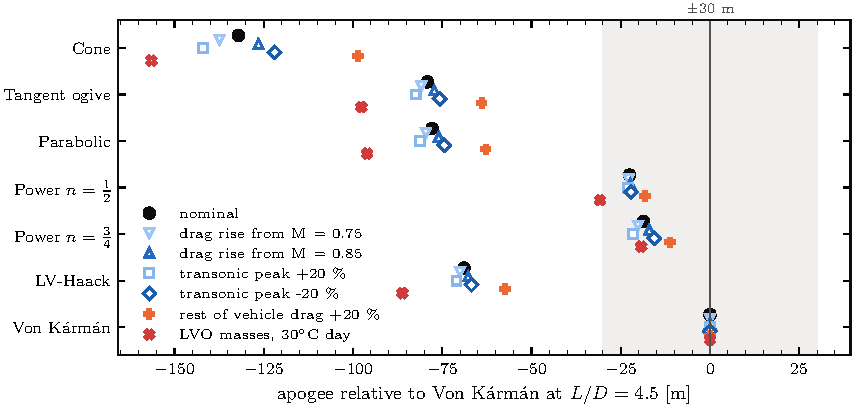
\includegraphics[width=\textwidth]{fig_robustness}
\caption{Apogee of each design at $L/D = 4.5$ relative to Von K\'arm\'an, under the nominal model
and six perturbed ones. The grey band is $\pm\SI{30}{m}$, about $\pm\SI{0.2}{kg}$ of dry mass.}
\label{fig:robustness}
\end{figure}

Each row of Figure~\ref{fig:robustness} is one design; the markers of a row are its apogee
deficit under the different models. The grey band marks differences of the order of the mass
uncertainty of a vehicle at this stage (\SI{0.2}{kg}); designs inside it are equivalent in
practice. Only the two power noses lie in it or at its edge, and no design crosses zero.

\subsection{Tip bluntness}
\label{sec:bluntness}

A sharp tip cannot be laid up and burns or chips first, so the tip is a separate machined
part. Figure~\ref{fig:bluntness}a gives the drag cost of a spherical tip on the Von K\'arm\'an
nose. At $M=1.4$ a \SI{4.5}{mm} tip ($r_n/R=0.05$) costs \BLUNTCOST{} (\BLUNTAPOA{} of apogee), and
a \SI{9}{mm} tip ($r_n/R=0.1$) costs \BLUNTTEN{} (\BLUNTAPOB{}). The cost grows quickly with radius because the
sphere replaces the slender front of the Haack profile.
Figure~\ref{fig:bluntness}b gives the benefit: the stagnation-point heat-transfer coefficient
falls as $r_n^{-1/2}$. The sphere is tangent to the profile and carries a small detached bow
shock (Section~\ref{sec:physics}). At its centre the pressure is the stagnation pressure behind a
normal shock, $C_p \approx 1.5$ at $M = 1.4$, against about 0.04 averaged over a sharp nose. The
penalty rises with Mach number because this stagnation pressure does. For the selected
\SI{4.5}{mm} tip, $h_s$ is about \SI{2}{kW/(m^2.K)}; doubling the radius would only lower it by
$\sqrt2$. A radius of \SI{4.5}{mm} therefore keeps the drag cost below 1\,\%, and the heating is
handled by the choice of tip material (Section~\ref{sec:heating}).

\begin{figure}[H]
\centering
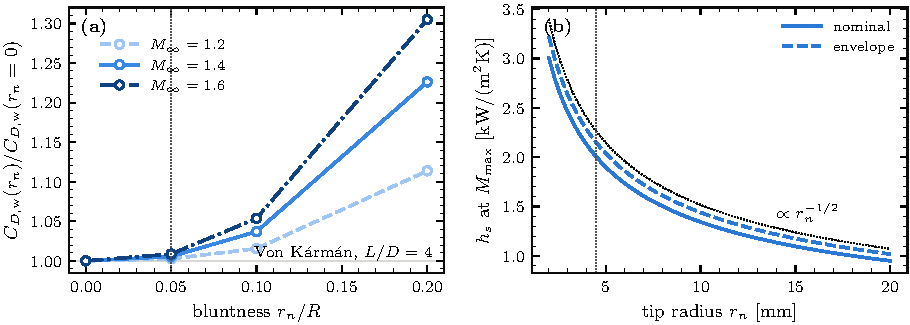
\includegraphics[width=\textwidth]{fig_bluntness}
\caption{(a) Wave drag of the blunted Von K\'arm\'an nose relative to the sharp one.
(b) Stagnation-point heat-transfer coefficient at $M_{\max}$ versus tip radius (dotted line: the
selected \SI{4.5}{mm}).}
\label{fig:bluntness}
\end{figure}

\subsection{Heating}
\label{sec:heating}

Figure~\ref{fig:thermal} gives the temperature histories. The peak stagnation temperature is
\SI{119}{\celsius} (nominal) and \SI{156}{\celsius} (envelope), reached at burn-out.
\begin{itemize}[leftmargin=*,itemsep=2pt]
\item \textbf{Tip.} A 3D-printed PET-CF tip (Firehorn) has a low conductivity, so its surface
follows $T_0$ and reaches \PETNOM{} (nominal) and \PETENV{} (envelope). That is
well above the \SIrange{70}{80}{\celsius} heat-deflection range of PET/PETG-CF. A
\SI{60}{g} Al 6082-T6 tip spreads the heat and stays below \TIPALNOM{} (nominal) and \TIPAL{} (envelope).
In the model PET-CF conducts heat 600 times less well than aluminium (\SI{0.3}{} against
\SI{180}{W/(m.K)}). The heat received at the surface of a printed tip stays in a thin layer, whose
temperature quickly approaches the recovery temperature. In the aluminium tip the same heat
spreads through the whole \SI{60}{g}, whose heat capacity limits the temperature rise. The
heat-deflection temperature (HDT) is the temperature at which a standard polymer specimen
deforms by a set amount under a set load; above it a printed tip would soften.
\item \textbf{Shell.} The \SI{1.2}{mm} CFRP shell follows the recovery temperature within a few
seconds. Its inner face peaks at \SHELLNOM{} (nominal) and \SHELLENV{} (envelope), about
\SI{3}{s} after burn-out, then cools. This is below the cure temperature of the prepreg, but the
envelope case comes close to the DP490 coupler bond (shear strength \SI{2.8}{MPa} at
\SI{120}{\celsius}). The Firehorn thermal requirement (\SI{390}{K} for \SI{5}{s}) does not
cover the envelope; Section~\ref{sec:next} proposes \SI{430}{K} for \SI{10}{s}. The inner face
peaks after burn-out because heat needs time to diffuse through the laminate: the outer surface
follows the recovery temperature, while the inner face lags behind it and keeps warming for a
few seconds after the outer surface has started to cool.
\end{itemize}

\begin{figure}[H]
\centering
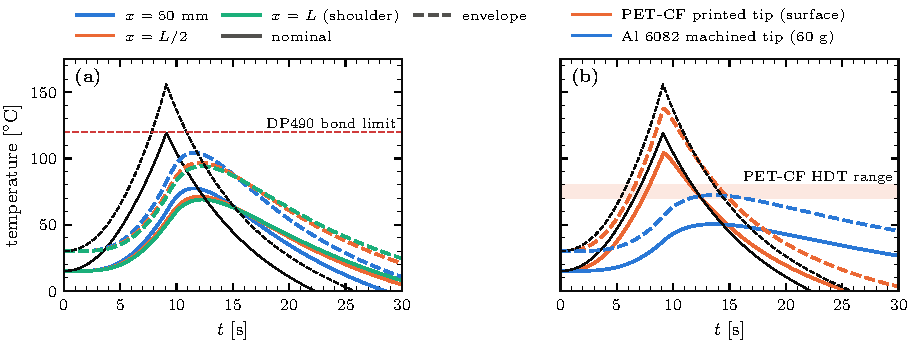
\includegraphics[width=\textwidth]{fig_thermal}
\caption{(a) Inner-face temperature of the CFRP shell at three stations (adiabatic inner face,
conservative). (b) Tip temperature: printed PET-CF surface against a machined Al 6082 insert.
Solid: nominal ascent; dashed: hot-day envelope; black: stagnation temperature $T_0$.}
\label{fig:thermal}
\end{figure}

Figure~\ref{fig:thermal} shows that heating is a material question, not a shape question. The
stagnation temperature is set by the trajectory, the same for every profile. What the design
controls is how much of it reaches a temperature-sensitive part, the tip polymer or the adhesive
bond. Both are protected by the choices made here: a metal tip and a thermal requirement that
covers the hot-day envelope.
